\documentclass[../analisi-dei-requisiti.tex]{subfiles}

\begin{document}
La presente sezione ha lo scopo di descrivere in maniera dettagliata, attraverso il linguaggio \glossario{UML}, le funzionalità offerte da \glossario{Stalker}.

\subsection{Attori dei casi d'uso}%
\label{sub:attori_casi_duso}

\subsubsection{Applicazione mobile}%
\label{subs:mobile_app}

\begin{figure}[H]
  \centering
  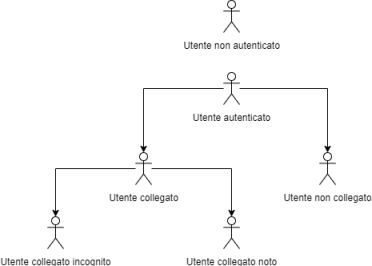
\includegraphics[width=100mm]{app_users.png}
  \caption{Utenti applicazione mobile}%
  \label{fig:usersapp}
\end{figure}

Un utente che accede per la prima volta all'applicazione mobile non è autenticato, quindi per accedere al sistema di Stalker inserisce le proprie credenziali per diventare un utente autenticato.
Successivamente a questo passaggio, l'utente è non collegato, in quanto subito dopo l'autenticazione non è collegato di default ad alcuna organizzazione. Nel momento in cui l'utente decida di collegarsi ad una o più organizzazioni, allora
diventa a tutti gli effetti un utente collegato che, in base al tipo di argomento dell'organizzazione scelta, può essere noto (con annessa autenticazione LDAP) se l'argomento dell'organizzazione è privato, altrimenti è incognito se l'argomento dell'organizzazione è pubblico.

\subsubsection{Web application}%
\label{subs:web_application}

\begin{figure}[H]
  \centering
  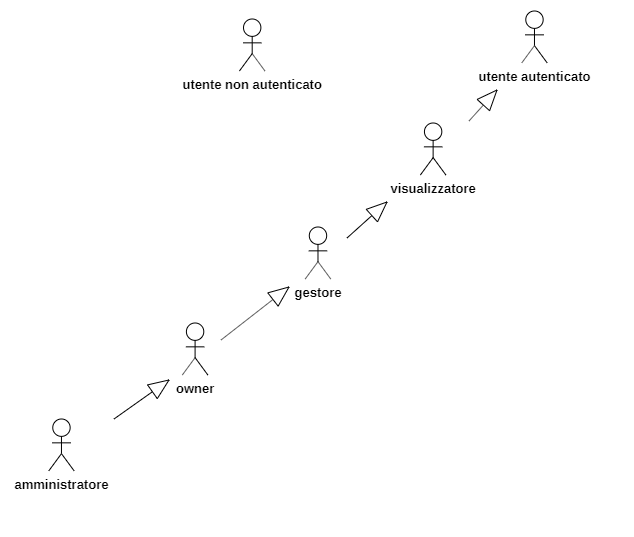
\includegraphics[width=100mm]{web_users.png}
  \caption{Utenti web application}%
  \label{fig:usersweb}
\end{figure}

Un utente che accede per la prima volta alla web application non è autenticato, quindi per accedere alla zona amministrativa di Stalker inserisce le
credenziali per diventare un utente autenticato.
Successivamente a questo passaggio, in base al tipo di privilegi l'utente può essere:
\begin{description}
  \item[visualizzatore]: visualizza determinate organizzazioni e i relativi luoghi, non ha permessi di modifica;
  \item[gestore]: gestisce i luoghi di una o più organizzazioni; eredita i privilegi del visualizzatore;
  \item[owner]: crea una o più organizzazioni, identificando i suoi gestori e visualizzatori; eredita i privilegi del gestore.
\end{description}
L'amministratore assume tutti i privilegi che il sistema può offrire, gestendo tutte le organizzazioni e i relativi owner, gestori e visualizzatori.

\end{document}
